\documentclass[12pt]{article}
\usepackage{fontspec}
\setmainfont{Times New Roman}
\usepackage{graphicx}
\usepackage{dirtree}
\usepackage{hyperref}
\usepackage{graphicx}
\usepackage{float}
\usepackage{enumitem}
\usepackage{caption}
\usepackage[%
    left=1.5cm,    % Narrower left margin
    right=1.5cm,   % Narrower right margin
    top=2cm,       % Reduced top space
    bottom=3cm,    % More footer space
    headheight=15pt,
    footskip=30pt
]{geometry}
\usepackage{listings}
\usepackage{xcolor}
\usepackage{tikz}
\usetikzlibrary{positioning,shapes,shadows,arrows}

\definecolor{myblue}{RGB}{80,80,160}
\definecolor{mygreen}{RGB}{80,160,80}

\lstset{
    basicstyle=\small\ttfamily,
    keywordstyle=\color{myblue}\bfseries,
    commentstyle=\color{mygreen},
    breaklines=true,
    showstringspaces=false
}

\title{\textbf{Project Proposal: Travel Agency Management System}}
\author{Peter Jiang \\ ID: 2430026079}
\date{\today}

\begin{document}

\maketitle

\section{Introduction}
This proposal outlines the implementation of a Travel Agency Management System (TAMS). The system streamlines operations for travel agencies by providing a comprehensive platform for managing travel bookings, itineraries, customer information, and other critical business operations. TAMS employs Object-Oriented Programming (OOP) principles, utilizes file I/O for data persistence, and features a user-friendly graphical interface built with Java Swing.

\section{Real-World Scenario and Business Logic}

\subsection{Scenario Overview}
The Travel Agency Management System serves the needs of modern travel agencies that offer various travel packages to different destinations. The agency handles customer bookings, maintains trip itineraries, manages payments, collects customer reviews, and organizes activities. This system digitizes these processes, enhancing operational efficiency and customer satisfaction.

\subsection{Business Logic}
The core business logic of the Travel Agency Management System includes:

\begin{itemize}
    \item \textbf{Package Management}: Create, update, and delete travel packages with details such as destination, duration, accommodations, activities, and pricing.
    
    \item \textbf{Customer Management}: Register new customers, update customer information, and track customer booking history.
    
    \item \textbf{Booking Process}: Allow customers to browse packages, make reservations, specify travel dates, and process payments.
    
    \item \textbf{Itinerary Management}: Create and modify detailed day-by-day itineraries for travel packages and custom trips.
    
    \item \textbf{Activity Management}: Maintain a database of activities that can be added to packages or itineraries.
    
    \item \textbf{Review System}: Collect and display customer reviews and ratings for travel packages.
    
    \item \textbf{Reporting}: Generate reports on bookings, revenue, customer statistics, and popular destinations.
\end{itemize}

\section{Object-Oriented Design}

\subsection{Class Hierarchy}
The system implements a comprehensive class structure that leverages key OOP concepts:

\begin{itemize}
    \item \textbf{Model Package}: Contains all data entities and business logic
    \begin{itemize}
        \item \texttt{TravelService}: Abstract class providing a base for travel offerings
        \item \texttt{TravelPackage}: Concrete implementation of a pre-defined travel package
        \item \texttt{CustomTrip}: Customized trip built for a specific customer
        \item \texttt{Customer}: User data and contact information
        \item \texttt{Booking}: Reservation details linking customers to travel packages
        \item \texttt{Payment}: Financial transaction details
        \item \texttt{Itinerary} and \texttt{ItineraryDay}: Trip timeline structure
        \item \texttt{Activity}: Individual activities that can be part of packages
        \item \texttt{Review}: Customer feedback and ratings
        \item \texttt{BookingStatus}, \texttt{PaymentMethod}, \texttt{PaymentStatus}: Enums for tracking status
        \item Interfaces: \texttt{Bookable}, \texttt{Reviewable}
    \end{itemize}
    
    \item \textbf{View Package}: GUI components
    \begin{itemize}
        \item \texttt{MainWindow}: Application container with tabbed navigation
        \item \texttt{BasePanel}: Abstract base for all panels
        \item \texttt{PackagesPanel}: Travel package management interface
        \item \texttt{TravelPackagesPanel}: Alternative package management view
        \item \texttt{CustomersPanel}: Customer data management
        \item \texttt{BookingsPanel}: Reservation processing
        \item \texttt{ActivitiesPanel}: Activity management
        \item \texttt{ReviewsPanel}: Customer feedback management
        \item \texttt{ReportsPanel}: Analytics and reporting
    \end{itemize}
    
    \item \textbf{Controller Package}: Application logic
    \begin{itemize}
        \item \texttt{TravelAgencyController}: Coordinates between views and model
    \end{itemize}
    
    \item \textbf{Util Package}: Utility services
    \begin{itemize}
        \item \texttt{DataManager}: Handles file I/O for data persistence
    \end{itemize}
    
    \item \textbf{Exceptions Package}: Custom exceptions
    \begin{itemize}
        \item \texttt{BookingException}: Booking-related errors
        \item \texttt{PaymentProcessException}: Payment processing errors
    \end{itemize}
\end{itemize}

\subsection{UML Class Diagram}

\begin{figure}[H]
\centering
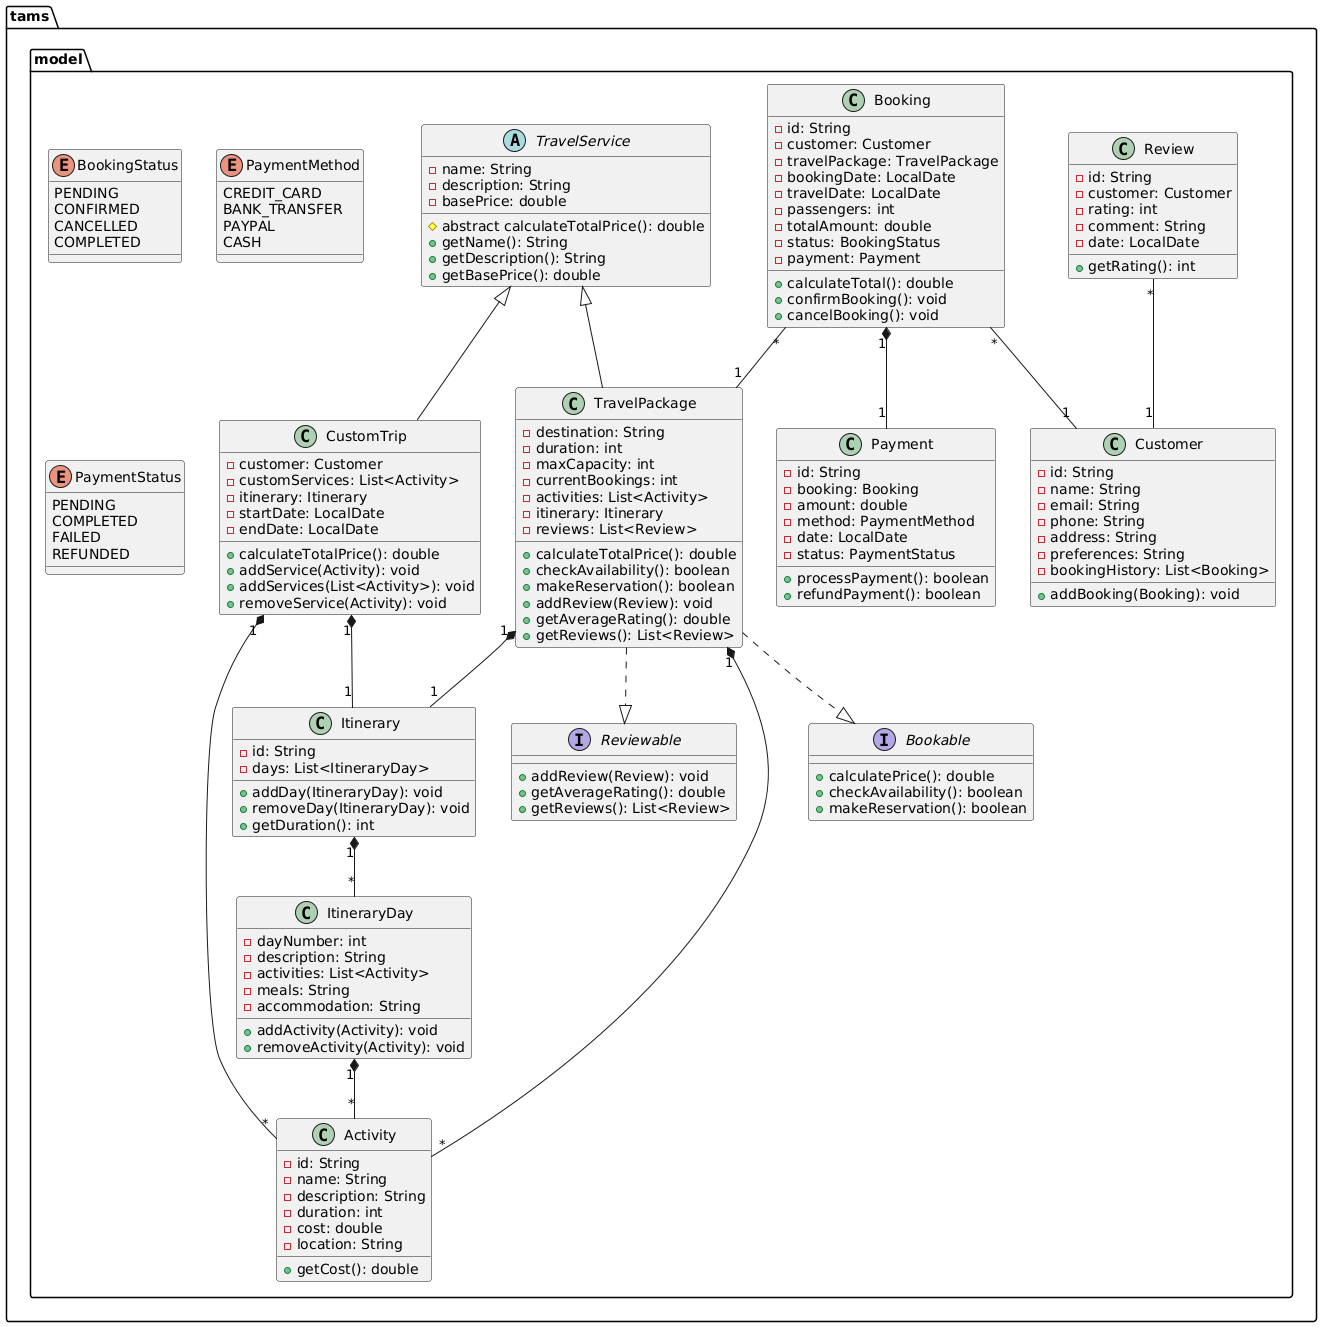
\includegraphics[width=\textwidth]{uml1.png}
\caption{Model}
\end{figure}
\newpage



\begin{figure}[H]
\centering
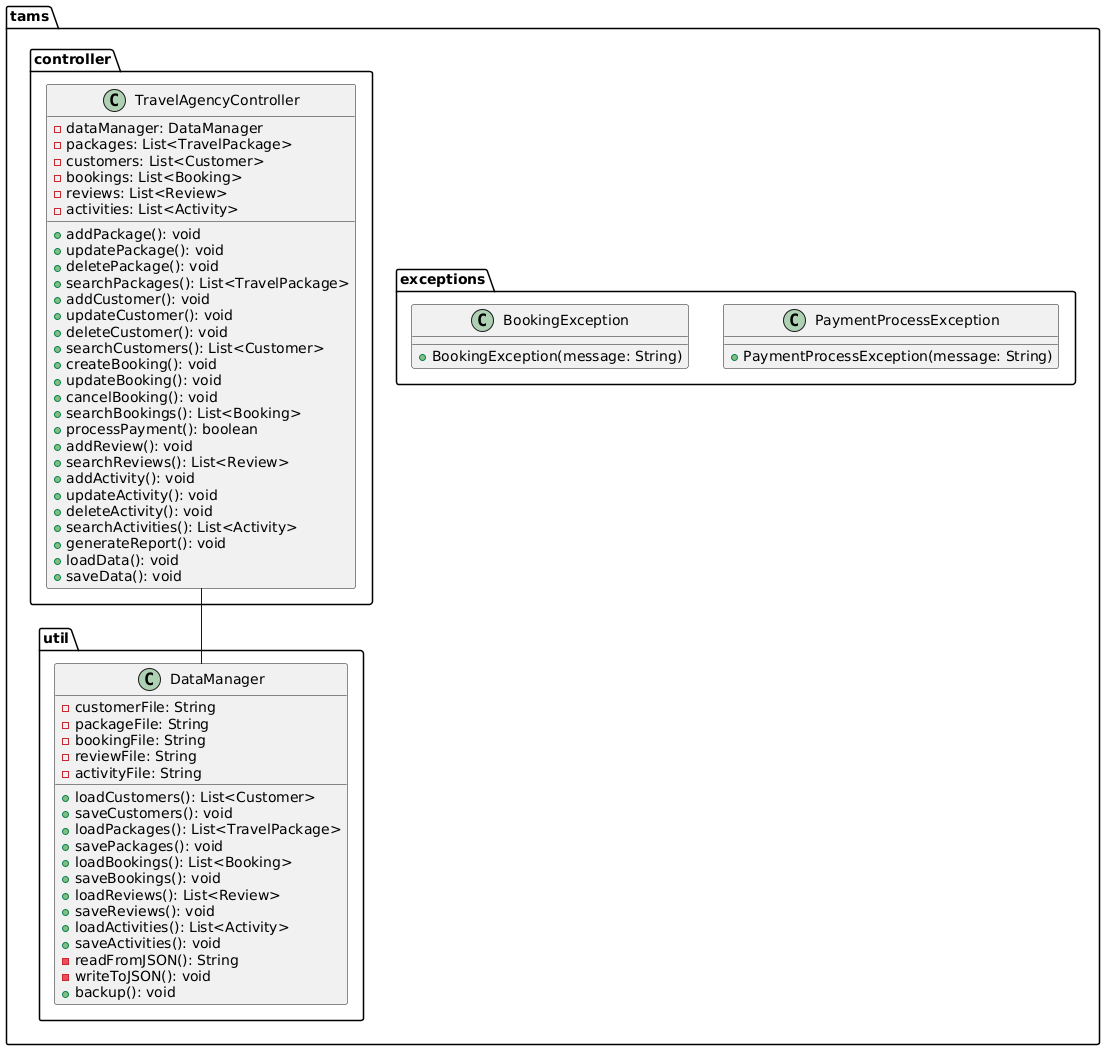
\includegraphics[width=\textwidth]{uml3.png}
\caption{Controller, Utilizes and Exceptions}
\end{figure}

\begin{figure}[H]
    \centering
    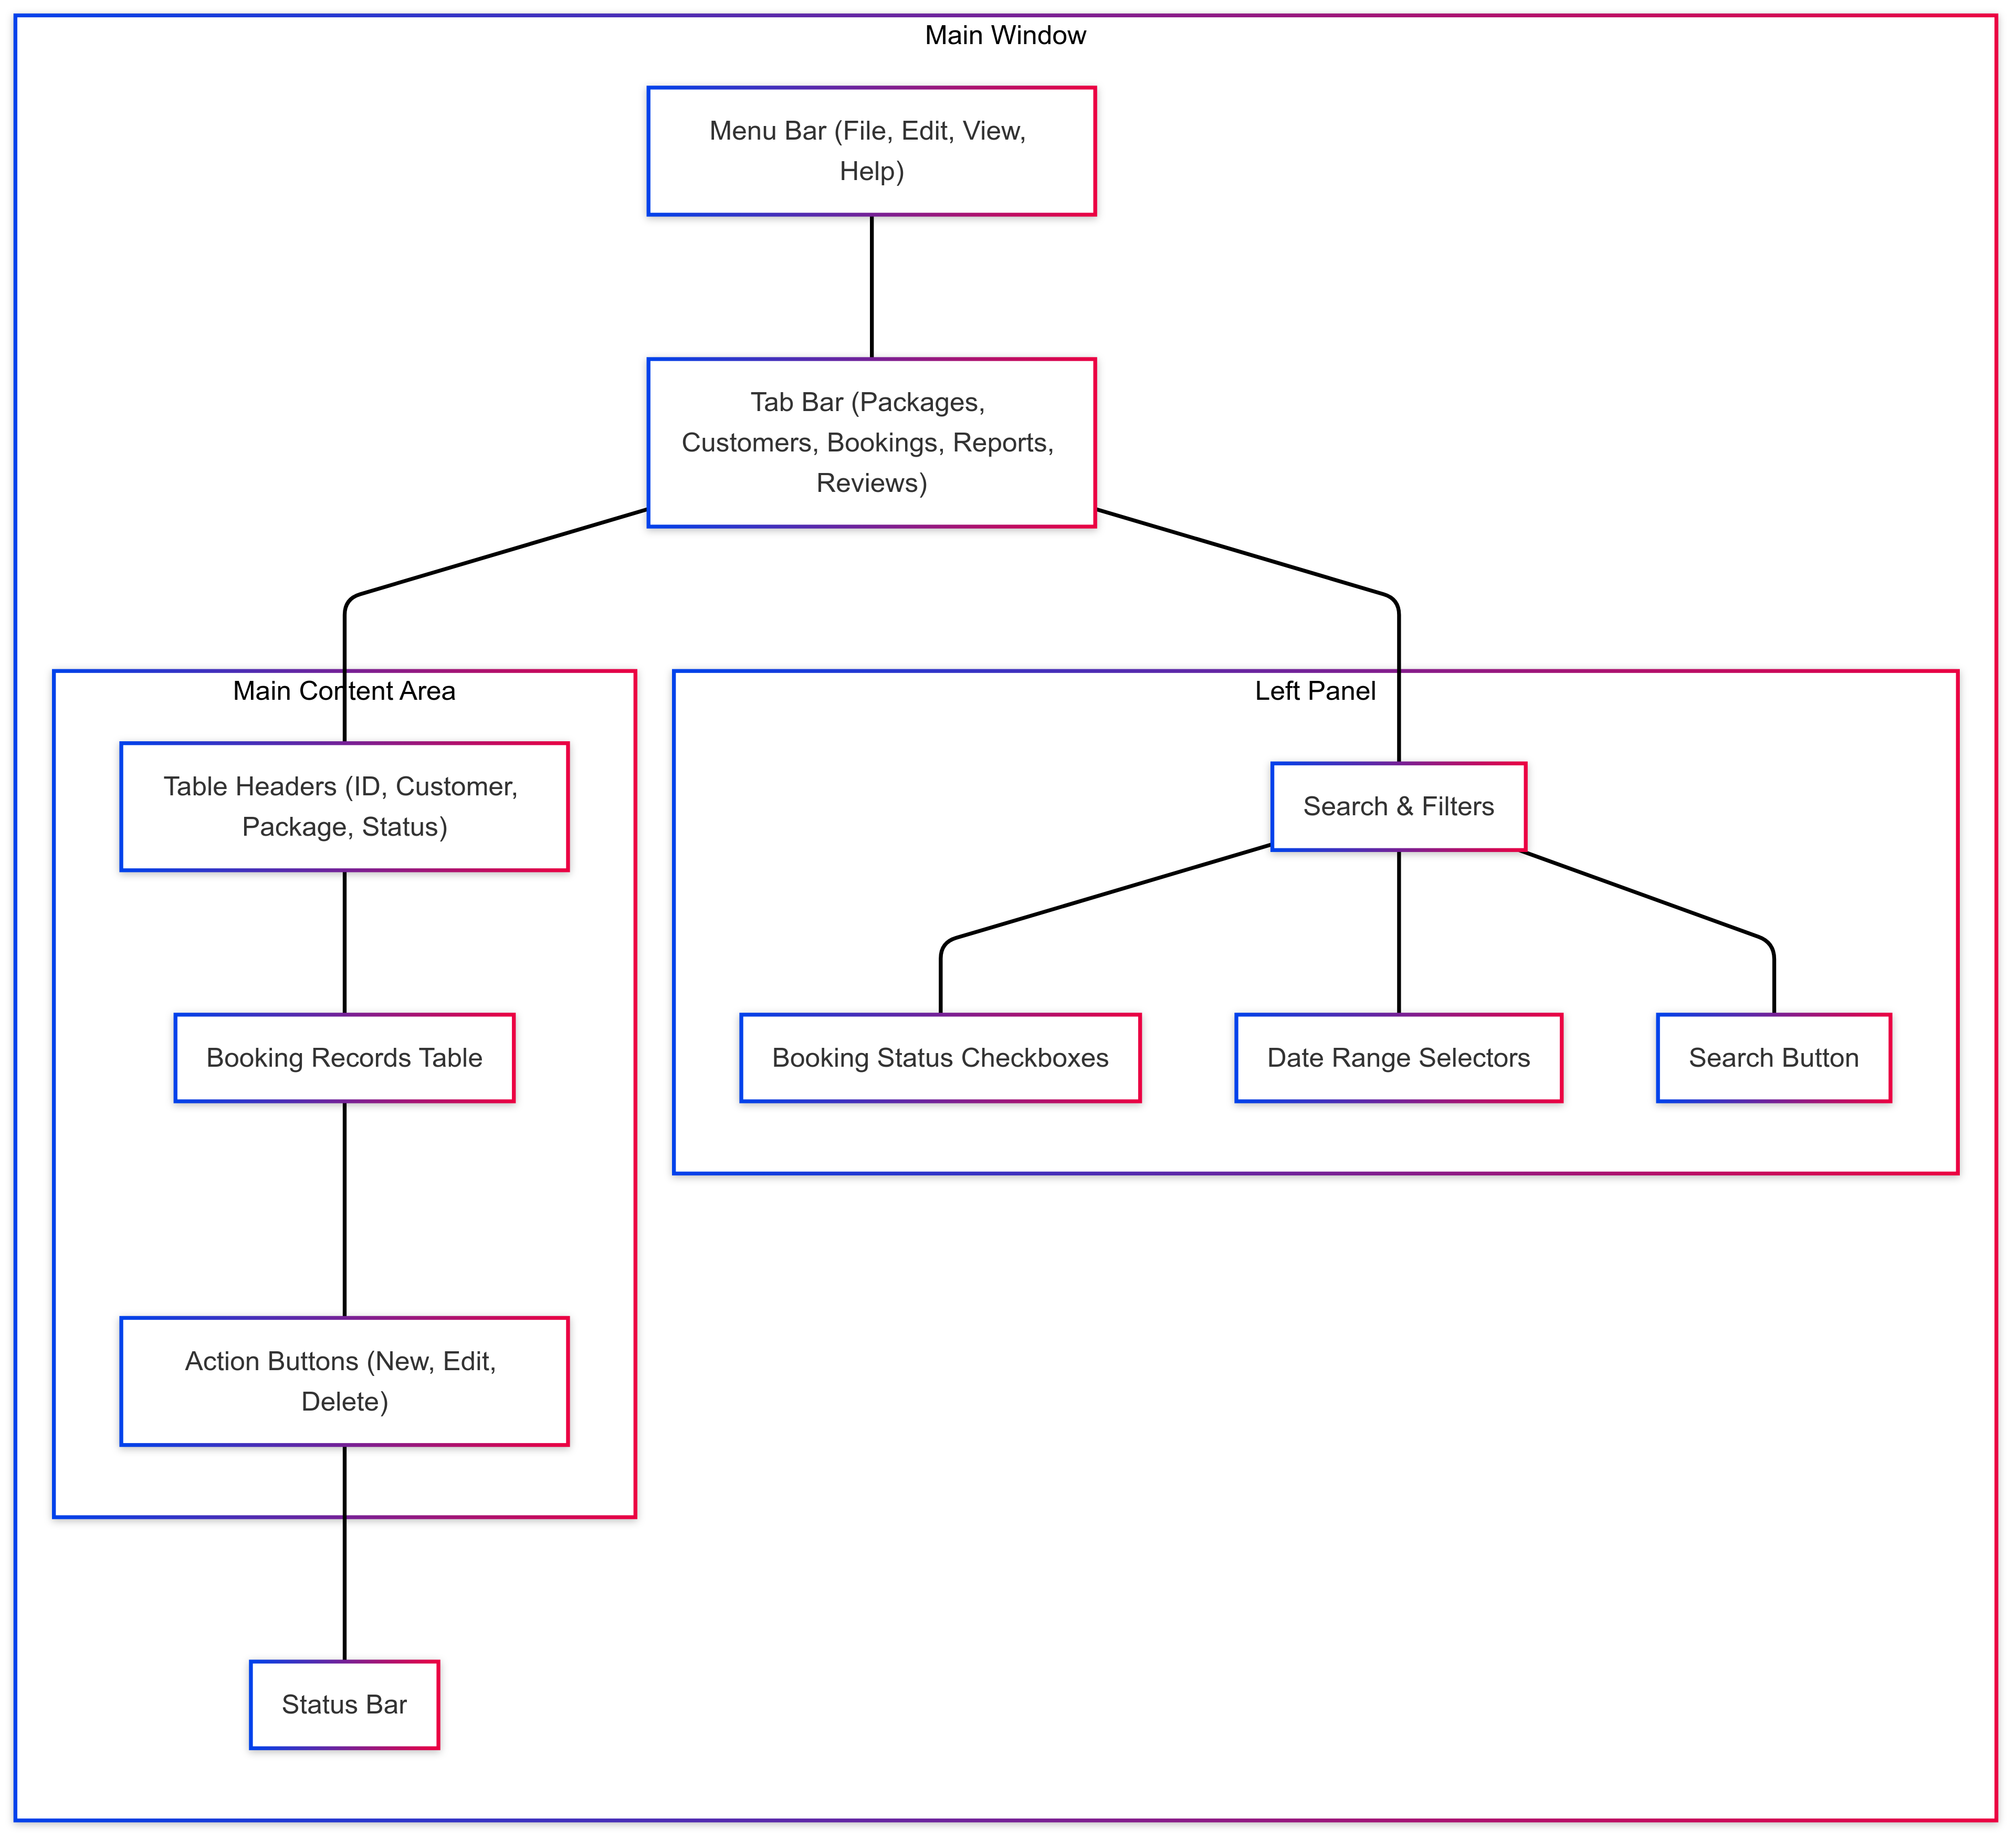
\includegraphics[width=\textwidth]{uml2.png}
    \caption{View}
    \end{figure}
\newpage

\subsection{OOP Concepts Implementation}

\subsubsection{Interfaces}
The system implements two main interfaces:

\begin{itemize}
    \item \textbf{Bookable}: Defines methods that any bookable service must implement, including \texttt{calculatePrice()}, \texttt{checkAvailability()}, and \texttt{makeReservation()}.
    
    \item \textbf{Reviewable}: Defines methods for entities that can receive customer reviews, including \texttt{addReview()}, \texttt{getAverageRating()}, and \texttt{getReviews()}.
\end{itemize}

\subsubsection{Abstract Classes}
\begin{itemize}
    \item \textbf{TravelService}: An abstract class that provides common attributes and methods for all travel services, including name, description, and base price. It includes abstract methods like \texttt{calculateTotalPrice()} that must be implemented by subclasses.
    
    \item \textbf{BasePanel}: Abstract class for all GUI panels, providing common functionality like setup methods, data refresh capabilities, and dialog handling to ensure consistent UI patterns.
\end{itemize}

\subsubsection{Inheritance}
The inheritance hierarchy includes:
\begin{itemize}
    \item \texttt{TravelService} serves as the parent class for \texttt{TravelPackage} and \texttt{CustomTrip}, allowing shared behavior while enabling specialized implementation.
    \item \texttt{BasePanel} is extended by all specific panels (\texttt{PackagesPanel}, \texttt{CustomersPanel}, etc.), providing common UI functionality.
    \item Each subclass inherits common attributes and methods while implementing specific behaviors.
\end{itemize}

\subsubsection{Polymorphism}
Polymorphism is demonstrated through:
\begin{itemize}
    \item Different implementations of \texttt{calculateTotalPrice()} in \texttt{TravelPackage} and \texttt{CustomTrip}.
    \item Use of the \texttt{Bookable} interface allowing different travel services to be treated uniformly.
    \item Panel-specific implementations of \texttt{refreshData()} and \texttt{setupUI()} methods.
    \item Ability to handle different types of travel services through a common parent class.
\end{itemize}

\subsubsection{Method Overloading}
\begin{itemize}
    \item Multiple constructors in classes like \texttt{Booking} and \texttt{Customer} with different parameter sets.
    \item \texttt{addService()} method in \texttt{CustomTrip} with versions for adding single services or collections.
    \item \texttt{searchPackages()} method in \texttt{TravelAgencyController} with different parameter combinations.
\end{itemize}

\subsubsection{Method Overriding}
\begin{itemize}
    \item Override of \texttt{calculateTotalPrice()} in subclasses of \texttt{TravelService}.
    \item Override of \texttt{toString()} in various model classes for customized string representation.
    \item Override of \texttt{refreshData()} in panel classes to update their specific content.
\end{itemize}

\subsubsection{Exception Handling}
Custom exceptions include:
\begin{itemize}
    \item \texttt{BookingException}: For handling errors in the booking process, such as unavailable packages or invalid booking details.
    \item \texttt{PaymentProcessException}: For managing payment processing errors, like failed transactions or invalid payment methods.
\end{itemize}
\newpage
\section{Graphical User Interface Design}

The GUI is implemented using Java Swing, providing an intuitive interface for users to interact with the system.
\subsection{GUI Examples}

\begin{figure}[H]
\centering
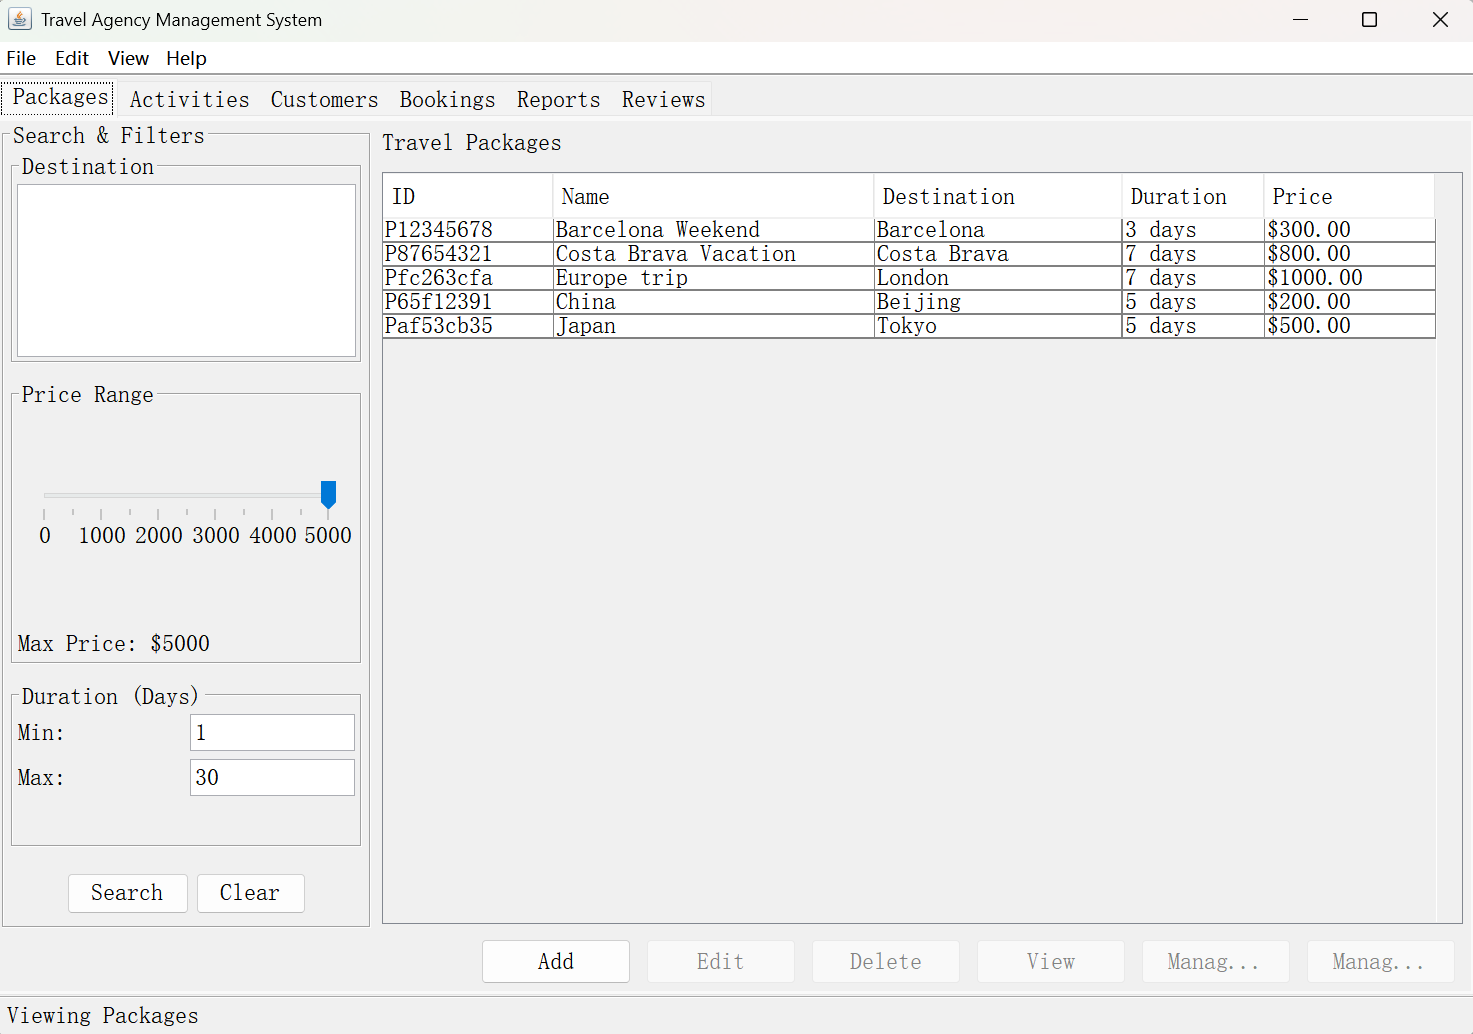
\includegraphics[width=\textwidth]{gui1.png}
\caption{Main Window (Packages Tab)}
\end{figure}

\begin{figure}[H]
\centering
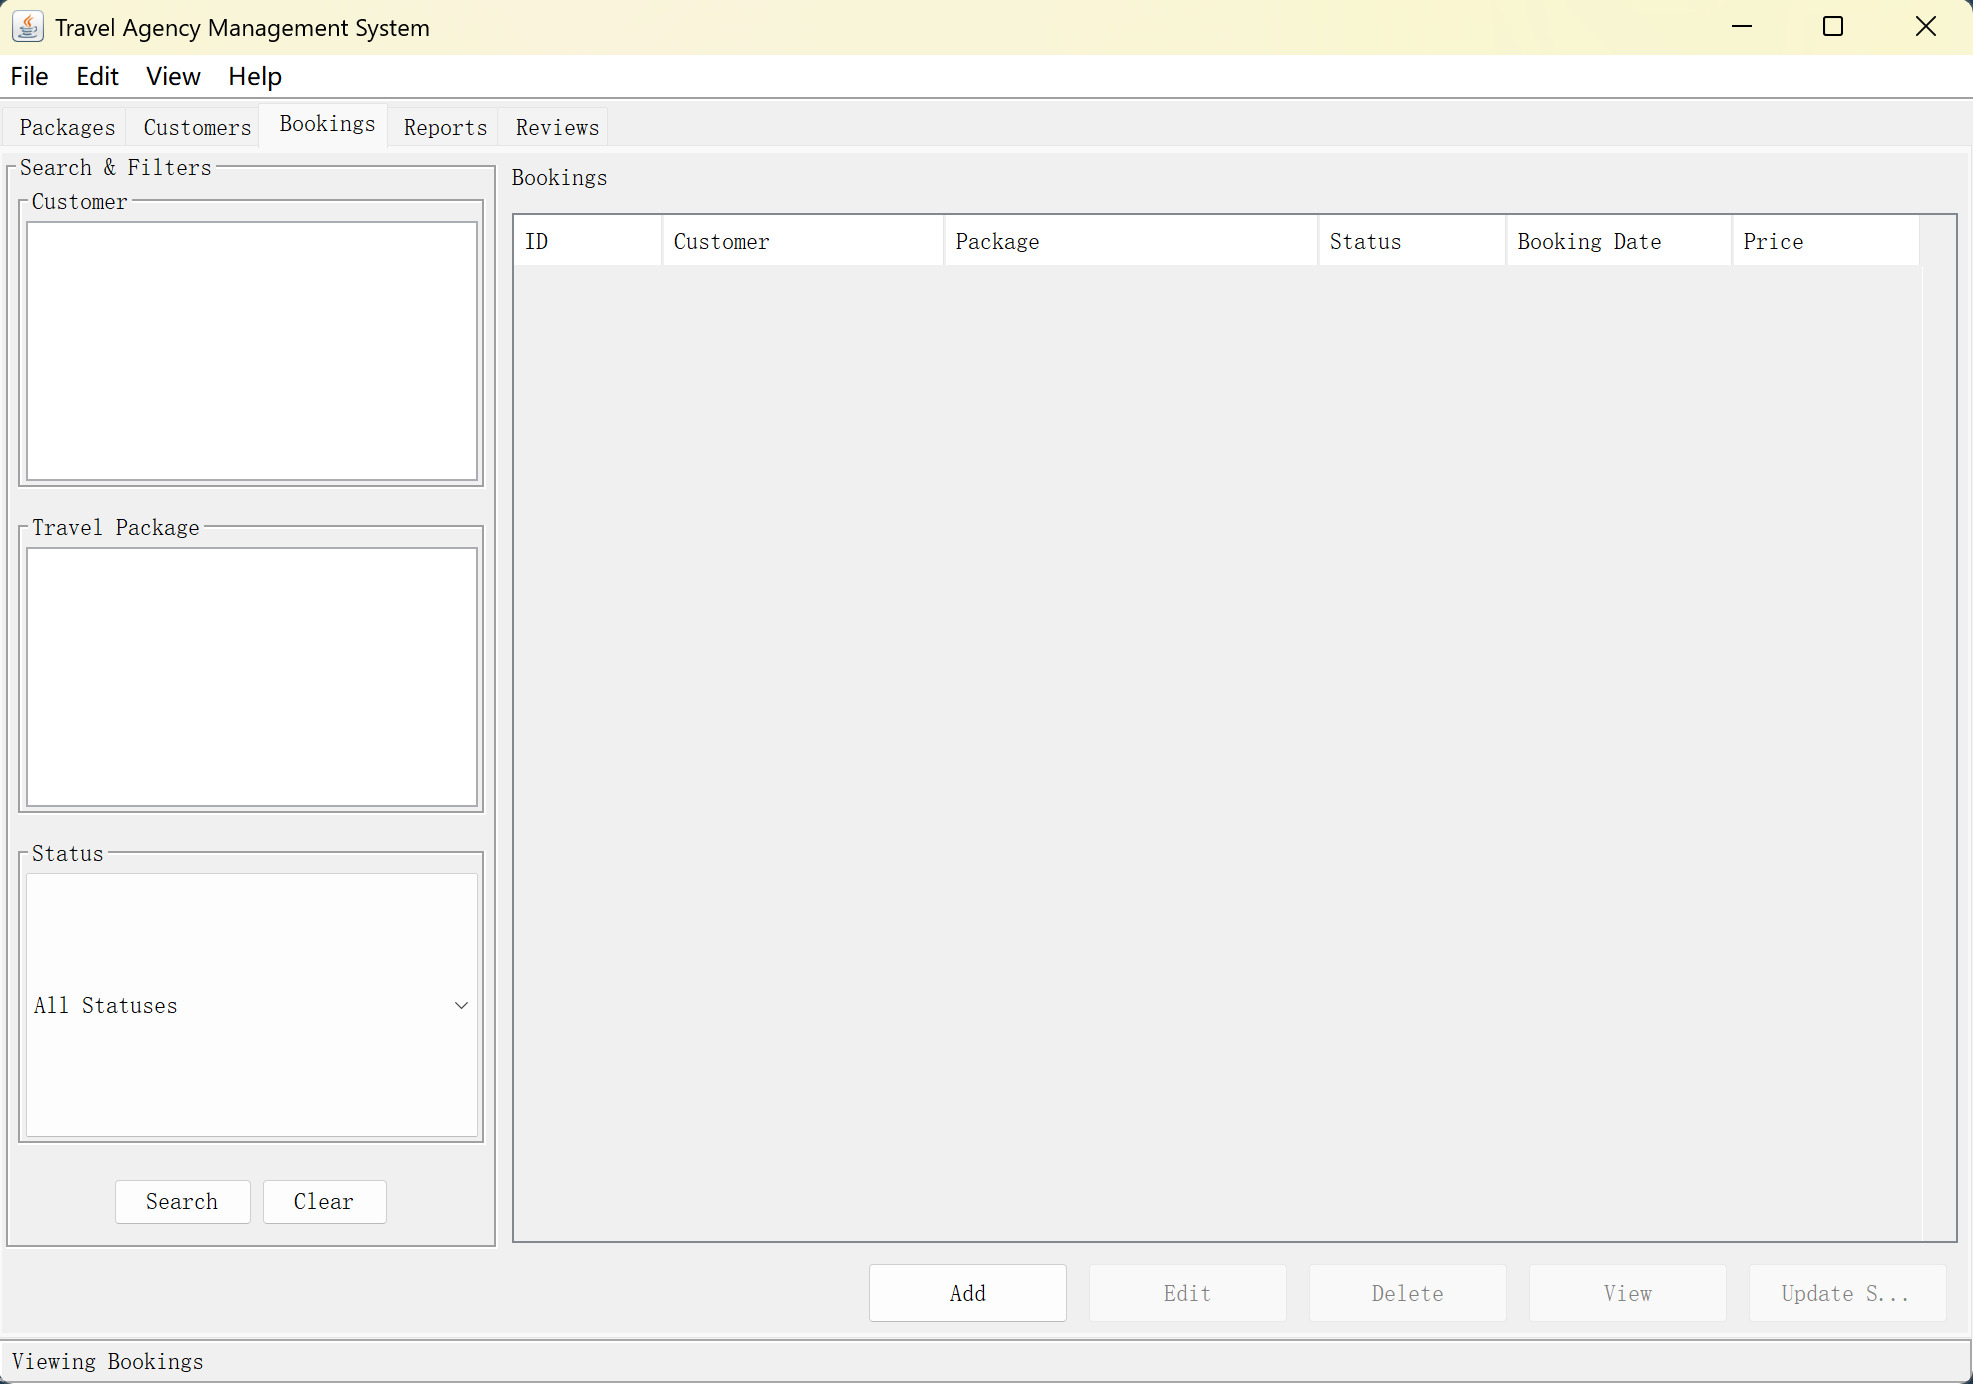
\includegraphics[width=\textwidth]{gui2.png}
\caption{Packages Panel (View packages detail)}
\end{figure}

\begin{figure}[H]
\centering
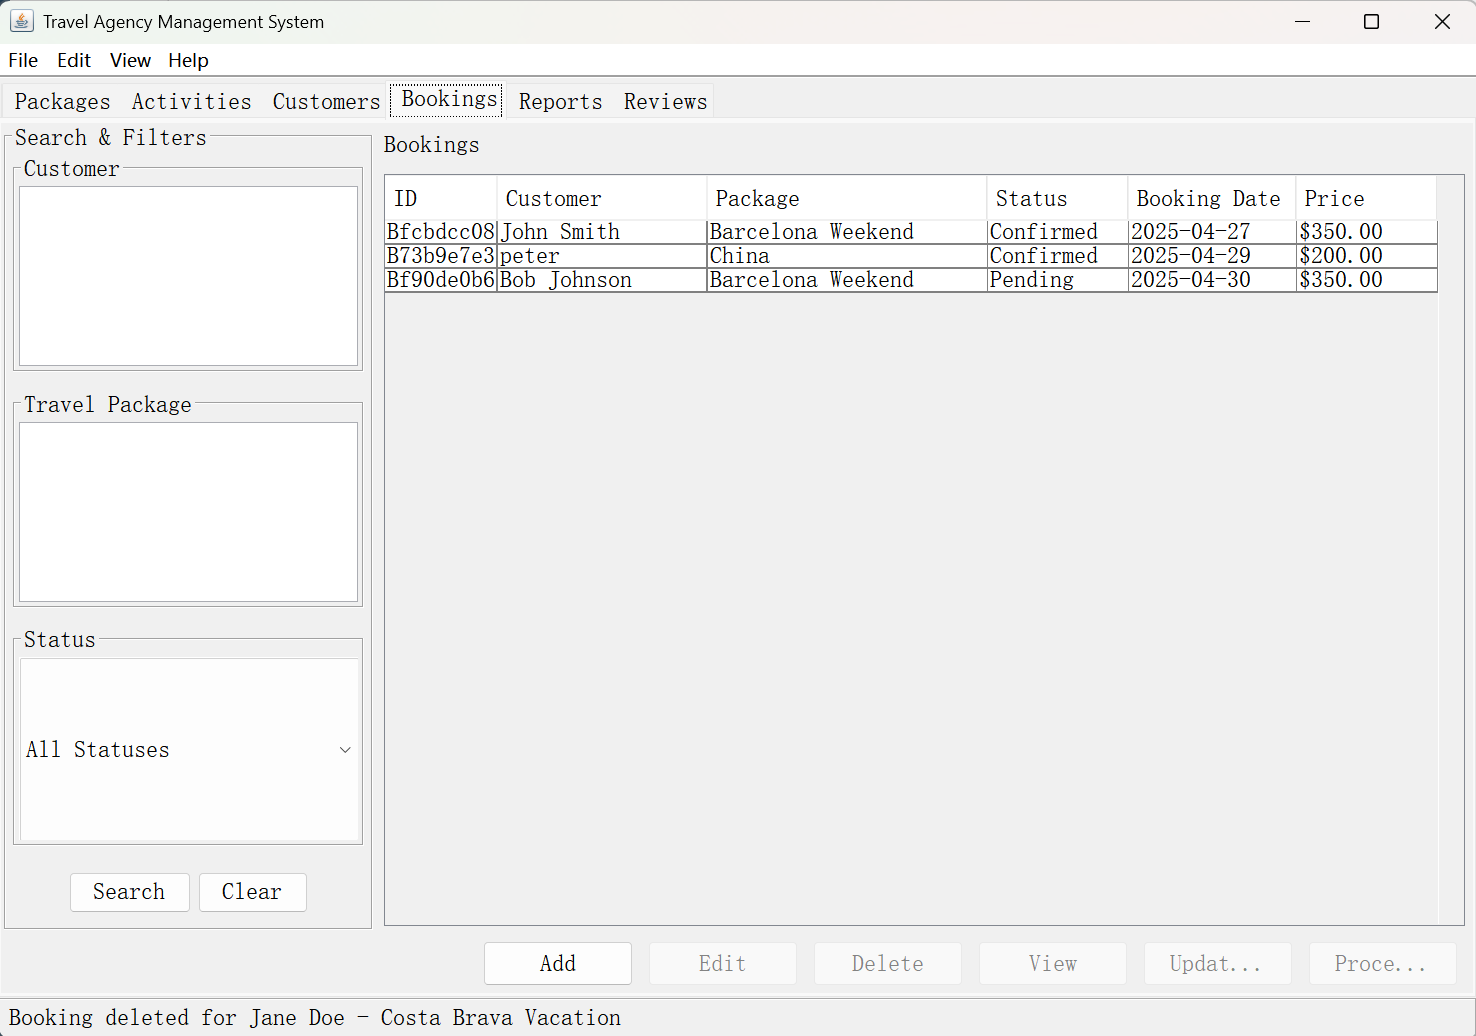
\includegraphics[width=\textwidth]{gui3.png}
\caption{Bookings Panel}
\end{figure}

The GUI implements the following features:

\begin{itemize}
    \item \textbf{Tab-based Navigation}: Easy navigation between different system functions through a tabbed interface:
    \begin{itemize}
        \item Packages Tab: For managing travel packages
        \item Customers Tab: For managing customer data
        \item Bookings Tab: For processing bookings
        \item Activities Tab: For managing activities
        \item Reviews Tab: For handling customer feedback
        \item Reports Tab: For analytics and reporting
    \end{itemize}
    
    \item \textbf{Search and Filtering}: Ability to search and filter data across all modules using text fields and dropdowns.
    
    \item \textbf{CRUD Operations}: Interface elements for creating, reading, updating, and deleting records:
    \begin{itemize}
        \item \textbf{Create}: Forms for adding new packages, customers, bookings, and activities
        \item \textbf{Read}: Tables and detailed views to display information
        \item \textbf{Update}: Forms to modify existing records
        \item \textbf{Delete}: Options to remove records with confirmation dialogs
    \end{itemize}
    
    \item \textbf{Reports Section}: Visual representation of data including:
    \begin{itemize}
        \item Booking statistics
        \item Revenue analysis
        \item Customer demographics
        \item Popular destinations and packages
    \end{itemize}
    
    \item \textbf{Interactive Elements}: Form controls including:
    \begin{itemize}
        \item Text fields for data entry
        \item Dropdown menus for selecting options
        \item Date pickers for scheduling
        \item Buttons for actions
        \item List components for displaying records
    \end{itemize}
\end{itemize}

\section{Data Storage Design}

\subsection{File I/O Architecture}
The system uses file I/O to store and retrieve data persistently. The data storage is organized as follows:

\begin{itemize}
    \item \textbf{JSON File Format}: Data is stored in JSON format for readability and ease of handling.
    
    \item \textbf{File Structure}:
    \begin{itemize}
        \item \texttt{customers.json}: Customer information and preferences.
        \item \texttt{packages.json}: Travel package details and availability.
        \item \texttt{bookings.json}: Booking records and status.
        \item \texttt{reviews.json}: Customer reviews and ratings.
        \item \texttt{activities.json}: Available activities for packages.
    \end{itemize}
    
    \item \textbf{Data Loading}: When the application starts, it loads data from these files into memory using the DataManager class.
    
    \item \textbf{Data Saving}: Changes are saved back to the files automatically when data is modified and when the application closes.
    
    \item \textbf{Data Validation}: Inputs are validated before being written to ensure data integrity.
\end{itemize}

\subsection{Data Processing}
The system includes:

\begin{itemize}
    \item \textbf{Data Validation}: Validating user inputs before saving to ensure data integrity.
    
    \item \textbf{Sorting and Searching}: Algorithms to efficiently sort and search through data collections.
    
    \item \textbf{Data Analysis}: Functions to analyze booking trends, popular destinations, and revenue statistics.
    
    \item \textbf{Data Export}: Capability to export reports for external use.
\end{itemize}

\section{Additional Features}

\subsection{Advanced Search Functionality}
The system includes advanced search options to:
\begin{itemize}
    \item Search packages by destination, date range, price range, or activities
    \item Filter customer records by name, email, or contact information
    \item Search bookings by status, date, or package type
    \item Find activities by location, type, or price range
\end{itemize}

\subsection{Data Analysis}
The system offers data analysis features:
\begin{itemize}
    \item Booking statistics and trends
    \item Popular destinations and activities
    \item Customer demographics and preferences
    \item Revenue analysis and projections
\end{itemize}

\section{Conclusion}
The Travel Agency Management System (TAMS) provides a comprehensive solution for travel agencies to manage their operations efficiently. By implementing the outlined features and following object-oriented design principles, the system offers a robust, user-friendly platform that enhances the agency's ability to serve customers and track business performance.

The system successfully meets all project requirements by implementing:
\begin{itemize}
    \item Multiple interfaces and abstract classes
    \item A robust inheritance hierarchy
    \item Polymorphic behavior for flexible operations
    \item Method overloading and overriding
    \item Custom exception handling
    \item Persistent data storage through file I/O
    \item A comprehensive Java Swing GUI
\end{itemize}

The modular design ensures that the system can be easily maintained and extended to accommodate future requirements and enhancements.

\section*{GitHub Repository}
The source code for this project is available at Github and I will keep updating it. If you have any question or feedback, please feel free to contact me at:\\
\href{https://github.com/jytpeterjiang/Travel-Agency-Management-System}{https://github.com/jytpeterjiang/Travel-Agency-Management-System}

\end{document}